%!TEX root = ../08-Interference.tex
\chapter{Newton's Rings}

The curvature radius of a biconvex lens and the refractive index of water are determined by analyzing the Newton's rings interference pattern of said lense.

\addsec{Setup}

Newton's rings is an interference phenomenon that occurs when a transparent spherical object is placed on a flat reflective surface and is illuminated from the top with monochromatic, coherent light.
A series of concentric rings can be observed.

Light is reflected on the top and bottom of the lens and substrate.
Inteference occurs between the light that is reflected on the bottom of the lens and the top of the substrate as shown in \autoref{fig:newton}.
The reflections that occur at the top of the lens and the bottom of the substrate do not produce interference patterns, as the path differences are much larger than the coherence length of tyical LEDs.

The two beams have a path difference of $2 d$. Additionally, a phase inversion occurs at the substrate, as the light enters a more optically dense medium.

The geometry of the spherical lens gives $d = \frac{r^2}{R}$, where $R$ is the curvature radius of the lens and $r$ is the horizontal radius from the contact point of the lens and substrate.

Substituting this into the condition for destructive interference $2 d \cdot n = k \lambda$ gives
\begin{equation}\label{eq:newton}
	\frac{r_k^2}{R} = \frac{k \lambda}{n} \quad \Leftrightarrow \quad \frac{r_k^2}{k} = \frac{R \lambda}{n},
\end{equation}
where $n$ is the index of refraction of the medium between the lens and substrate.
The ratio $\frac{r_k^2}{k}$ is constant, it can be determined using linear regression.

A microscope slide is used as the substrate.
The lens and substrate are placed in a microscope with an XY-stage and a vernier scale on both axes.
The rings are centered around the crosshair.
A crosshair is used to find the edges of the rings along one axis, the rings' radii are read on the vernier scale.

To shorten the calculations, the refractive index of air is assumed to be exactly \num{1}.

\begin{figure}[tbp]
	\centering
	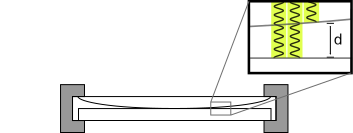
\includegraphics[width=.6\textwidth]{img/newtons-rings.pdf}
	\caption{Newton's Rings}
	\label{fig:newton}
	\caption*{based on \url{https://en.wikipedia.org/wiki/Newton\%27s_rings\#/media/File:Newton\%27s_rings_02.svg}}
\end{figure}

\section{Measuring the Radius of Curvature}\label{sec:radius}

\begin{figure}[tbp]
	\centering
	\begin{subfigure}{.49\textwidth}
		\centering
		\includegraphics[width=1.1\textwidth]{data/plots/1-1-blue.pdf}
		\caption{Blue LED (\SI{465}{\nm})}
		\caption*{$\frac{r_k^2}{k} = \SI{0.154}{\mm\squared}$}
	\end{subfigure}
	\begin{subfigure}{.49\textwidth}
		\centering
		\includegraphics[width=1.1\textwidth]{data/plots/1-1-yellow.pdf}
		\caption{Yellow LED (\SI{590}{\nm})}
		\caption*{$\frac{r_k^2}{k} = \SI{0.173}{\mm\squared}$}
	\end{subfigure}
	\caption{Newton's Rings in Air}
	\label{fig:newton-air}
\end{figure}

Radii for rings of all discernible orders are measured with yellow and blue light.
The measured values for $r_k^2$ are plotted in \autoref{fig:newton-air}.
Solving \autoref{eq:newton} for $R$ and substituting the wavelengths and slopes of the lienar fits, this yields $R_\text{blue} = \SI{0.33}{\meter}$ and $R_\text{yellow} = \SI{0.29}{\meter}$.

\section{Refractive Index of Water}

The experiment is repeated with yellow light and water between the substrate and lens.
The slope of the linear fit is $\frac{r_k^2}{k} = \SI{0.146}{\mm\squared}$ giving an uncorrected radius of $R_\text{water} = \SI{0.25}{\meter}$.
To increase accuracy, both measurements from \autoref{sec:radius} are averaged to form the reference value.
The radii of curvature $R$ are used instead of the slopes, as they are independent of the wavelength, the average radius in air is $\langle R_\text{air} \rangle = \SI{0.31}{\meter}$.

The index of refraction of water is calculated as
\begin{equation*}
	n_\text{water} = \frac{\langle R_\text{air} \rangle}{R_\text{water}} = \num{1.26},
\end{equation*}
which deviates from the literature value of $n_\text{lit,water} = \num{1.33}$ by \SI{5}{\percent}.

\section{Focal Length of the Lens}

The focal length of the lens is determined by autocollimation.
A light source, a transparent screen with an opaque pattern, the lens used in the previous experiments and a planar mirror are placed on an optical bench.
When the distance between the screen and lens matches its focal length, all light rays coming from a single point on the screen will leave the lens parallel.
The parallel beams are reflected back through the lens by the mirror and are focused to a single point on the screen.
The distance between lens and mirror does not affect the results.
However, it has to be made sure that for small distances between lens and screen, the lens might reflect the pattern onto the screen again, which could trick someone into thinking, they've found the focal point, without this actually being the case.
This can be checked for by holding a hand into the beam between lense and mirror and making sure, the image of the pattern disappears.

The focal length of the lens used is determined to be $f = \SI{290}{\mm}$.

\section{Refractive Index of the Lens}
The geometry of a plano-convex lens (\autoref{fig:lens}) and Snell's law give
\begin{gather*}
	\sin(\alpha) = \frac{h}{R}, \quad\;
	\tan(\gamma) = \frac{h}{f}, \quad\;
	\beta = \alpha + \gamma \quad \text{and} \quad
	n \sin(\alpha) = n_\text{L} \sin(\beta),
\end{gather*}
which can be simplified for small angles and combined to form $R = \left(n - 1\right)f$.
Binconvex lenses have twice the refractive power, which translates to
\begin{equation*}
	R = 2 \left(n - 1\right)f.
\end{equation*}

Using the previously measured values for $R$ and $f$, this gives an index of refraction of $n = \num{1.53}$.
Most glass blends have an index of refraction of \num{\sim 1.5} which is very close to the result.
The exact type of glass used is unknown, so a quantitative comparison is not possible.

\begin{figure}[tbp]
	\centering
	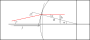
\includegraphics[width=.6\textwidth]{img/lens.pdf}
	\caption{Lens Focal Length}
	\label{fig:lens}
\end{figure}
